\documentclass[a4paper,10pt]{article}
\usepackage[utf8]{inputenc}
\usepackage[spanish]{babel}
\usepackage[affil-it]{authblk}
\usepackage{enumerate}
\usepackage{graphicx}
\usepackage{hyperref}
\usepackage{amsmath}
\usepackage{amssymb}
\usepackage{cancel}
\usepackage[usenames, dvipsnames]{color}
\usepackage{tikz}
\usepackage[labelfont=bf]{caption}
\usepackage{subcaption} %Multiple images
\usepackage{multicol} % Multiple columns
\usepackage{float}
\usepackage{cleveref}
 \usepackage{relsize} % bigger math symbols
\usepackage[margin=1.4in]{geometry}
\usepackage[titletoc,toc,title]{appendix}
\usepackage{enumitem}
\usepackage{etoolbox}
\usepackage{mdframed} %frame theorems
\usetikzlibrary{calc}
\numberwithin{equation}{section}

% Enviroment for theorems
\newmdtheoremenv[frametitle=Teorema]{theo}{Theorem}

% Circled words
\newcommand{\circled}[2][]{%
  \tikz[baseline=(char.base)]{%
    \node[shape = circle, draw, inner sep = 1pt]
    (char) {\phantom{\ifblank{#1}{#2}{#1}}};%
    \node at (char.center) {\makebox[0pt][c]{#2}};}}
\robustify{\circled}

%Appendices in spanish
\renewcommand{\appendixname}{Ap\'endices}
\renewcommand{\appendixtocname}{Ap\'endices}
\renewcommand{\appendixpagename}{Ap\'endices}

%Zero delimiter
\newcommand{\zerodel}{.\kern-\nulldelimiterspace}

%Columns separation
\setlength{\columnsep}{1cm}

%Indentation
\setlength{\parindent}{0ex}

%Multiple References

\crefrangelabelformat{equation}{(#3#1#4--#5\crefstripprefix{#1}{#2}#6)}

\usepackage{xparse}

%Boxes

\newcommand*{\boxcolor}{blue}
\makeatletter
\renewcommand{\boxed}[1]{\textcolor{\boxcolor}{%
\tikz[baseline={([yshift=-1ex]current bounding box.center)}] \node [rectangle, minimum width=1ex,rounded corners,draw] {\normalcolor\m@th$\displaystyle#1$};}}
 \makeatother

%Constantes
\newcommand{\euler}{\mathrm{e}}
\newcommand{\im}{i}

%Lemas, teoremas, definiciones y pruebas
\newcommand{\definicion}{\textbf{Definición: }}
\newcommand{\lema}{\textbf{Lema: }}
\newcommand{\teorema}{\textbf{Teorema: }}
\newcommand{\prueba}{\textbf{Prueba: }}
\newcommand{\proposicion}{\textbf{Proposición: }}
\newcommand{\corolario}{\textbf{Corolario: }}

% Definición de las secciones y su numeración

\makeatletter
\def\@seccntformat#1{%
  \expandafter\ifx\csname c@#1\endcsname\c@section\else
  \csname the#1\endcsname\quad
  \fi}
\makeatother

%opening
\title{Mecánica Clásica Tarea \# 14}
\author{Favio Vázquez\thanks{Correo: favio.vazquezp@gmail.com}}\affil{Instituto de Ciencias Nucleares. Universidad Nacional Autónoma de México.}
\date{}

\begin{document}

\makeatletter
\def\@maketitle{%
  \newpage
  \null
  \vskip 2em%
  \begin{center}%
  \let \footnote \thanks
    {\Large\bfseries \@title \par}%
    \vskip 1.5em%
    {\normalsize
      \lineskip .5em%
      \begin{tabular}[t]{c}%
        \@author
      \end{tabular}\par}%
    \vskip 1em%
    {\normalsize \@date}%
  \end{center}%
  \par
  \vskip 1.5em}
\makeatother

\maketitle

\section{Problema 1}

Utilizando únicamente la ecuación de la eikonal deduzca la ley de Snell.

\vspace{.3cm}

\underline{Solución:} \vspace{.3cm}

Recordemos la expresión para la ecuación de la eikonal,

\begin{equation}
 |\nabla S|^2(\mathbf{r}) = n^2(\mathbf{r}).
\end{equation}

Esta ecuación es simplemente el módulo de la ecuación de Huygens que puede 
escribirse como 

\begin{equation}
 \nabla S = n(\mathbf{r})\hat{\mathbf{s}},
\end{equation}

y también sabemos que el gradiente de esta ecuación define el vector de rayo de 
magnitud $|\mathbf{n}| = n$. Si ahora recordamos que la integración del gradiente 
sobre un camino cerrado se hace cero, tenemos que 

\begin{equation}
\oint_P \nabla S(\mathbf{r}) \cdot d\mathbf{r} = \oint_P \mathbf{n}(\mathbf{r}) 
\cdot d\mathbf{r} = 0.
\end{equation}

Consideremos ahora el caso en que el camino cerrado $P$ rodea una frontera que 
separa dos medios diferentes. Si hacemos que los lados del bucle perpendicular 
a la interfaz vayan a cero, entonces únicamente las partes de la integral de línea 
tangenciales al camino de la interfaz contribuirán en la misma. Ahora debido a que 
estas contribuciones deben sumar cero, las componentes tangenciales de los vectores 
de rato deben preservarse, esto es 

\begin{equation}
 (\mathbf{n} - \mathbf{n}') \times \hat{\mathbf{z}} = 0,
 \label{eq:preservacionTangencial}
\end{equation}

donde el primo se refiere al lado de la frontera al cual el rayo es transmitido, 
cuyo vector normal es $\hat{\mathbf{z}}$. Ahora imaginemos a un rayo atravesando 
la frontera y pasando a través de la región encerrada por el bucle de integración. 
Si $\theta$ y $\theta'$ son los ángulos de incidencia y transmisión, respectivamente, 
medidos desde la normal $\hat{\mathbf{z}}$ a través de la frontera, entonces la 
preservación de la componente tangencial del vector de rayo significa que, 
tomando en cuenta \eqref{eq:preservacionTangencial} y la definición del 
producto vectorial,

\begin{equation}
 \mathbf{n} \times \hat{\mathbf{z}} - \mathbf{n}' \times \hat{\mathbf{z}} = 0,
\end{equation}

\begin{equation}
 n\sen{\theta} - n'\sen{\theta'} = 0,
\end{equation}

esto debido a que $|\hat{\mathbf{z}}| = 1$, por lo tanto 

\begin{equation}
 \boxed{n\sen{\theta} = n'\sen{\theta'}.}
\end{equation}

Que es la ley de la refracción de Snell, descubierta primero por Ibn Sahl en 984 \cite{rashed}, 
y luego por Willebrod Snellius en 1621 \cite{holm}. Un análisis similar puede aplicarse al 
caso de los rayos reflejaos para mostrar que el ángulo de incidencia debe ser igual 
al ángulo de reflexión.

\section{Problema 2}

En el curso se mostró que la ecuación de la eikonal es una aproximación de onda 
pequeña de la ecuación de ondas. Encuentre ahora, a partir únicamente del principio 
de Fermat, las ecuaciones diferenciales que determinan los rayos de luz y la ecuación 
de la eikonal. Comente sobre la situación análoga entre las ecuaciones de movimiento 
de la mecánica y el principio de Hamilton.

\vspace{.3cm}

\underline{Solución:} \vspace{.3cm}

En gran parte esta discusión y pruebas fueron tomadas de \cite{holm}. Matemáticamente, el principio de Fermat establece que el camino un rayo $\mathbf{r}(s)$ 
de un punto $A$ a un punto $B$ en el espacio es un extremal de la longitud óptica, 
definida por 

\begin{equation}
 \delta \int_A^B n(\mathbf{r}(s)) = 0.
\end{equation}

Donde $n(\mathbf{r})$ es el índice de refracción en el punto espacial $\mathbf{r}$ 
y 

\begin{equation}
 ds^2 = d\mathbf{r}(s) \cdot d\mathbf{r}(s)
\end{equation}

es el elemento de la longitud de arco $ds$ a lo largo del camino del rato $\mathbf{r}(s)$ 
a través del punto.

\vspace{.3cm}

\definicion El \textbf{eje óptico} se define como la dirección principal de propagación de la 
luz. 

\vspace{.3cm}

Si se escogen coordenadas de manera que el eje $z$ coincida con el eje óptico y 
se exprese el elemento de longitud de arco $ds$ en términos del incremento a lo 
largo del eje óptico, $dz$, como 

\begin{align*}
 ds &= \left[(dx)^2 + (dy)^2 + (dz)^2 \right]^{1/2}\\
    &= \left[1 + \dot{x}^2 + \dot{y}^2 \right]^{1/2} = \frac{1}{\gamma}dz,
\end{align*}

donde hemos utilizado la notación $\dot{x} \equiv dx/dz$, $\dot{y} \equiv dy/dz$ y 
$\gamma \equiv dz/ds$, entonces el principio de Fermat puede interpretarse como 
un principio de acción estacionaria, con $z$ jugando el papel del tiempo (de aquí 
en adelante escribiremos $t$ en vez de $z$),

\begin{equation}
 0 = \delta S \equiv \delta \int_{t_A}^{t_B} L(x,y,\dot{x},dot{y},t)dt.
 \label{eq:112}
\end{equation}

Aquí, hemos definido la lagrangiana óptica como 

\begin{equation}
 L(x,y,\dot{x},dot{y},t) = n(x,y,t)\left[1 + \dot{x}^2 + \dot{y}^2 \right]^{1/2} = 
 \frac{n(x,y,t)}{\gamma},
\end{equation}

con 

\begin{equation}
 \gamma \equiv \frac{1}{\sqrt{1 + \dot{x}^2 + \dot{y}^2}} \leq 1.
\end{equation}

Podemos pensar en $(x,y,t) = (\mathbf{q},t)$ donde $\mathbf{q} = (x,y)$ es un vector 
con componentes en el plano perpendicular al eje óptico a un desplazamiento en un 
tiempo $t$. En esta formulación, el principio de Fermat implica la ecuación 
eikonal, lo cual establecemos en el siguiente teorema:

\vspace{.3cm}

\begin{mdframed}[linewidth=2]

\teorema El principio de Fermat

\begin{equation}
 0 = \delta S = \delta \int_{t_A}^{t_B} L(\mathbf{q}(t),\dot{\mathbf{q}}(t))dt, 
\end{equation}

para la lagrangiana óptica 

\begin{equation}
 L(\mathbf{q},\dot{\mathbf{q}},t) = n(\mathbf{q},t)\left[1 + |\dot{\mathbf{q}}|^2
 \right]^{1/2} \equiv \frac{n}{\gamma},
 \label{eq:113}
\end{equation}

con 

\begin{equation}
 \gamma \equiv \frac{dt}{ds} = \frac{1}{\sqrt{1 + |\dot{\mathbf{q}}|^2}} \leq 1,
 \label{eq:114}
\end{equation}

implica la ecuación de la eikonal

\begin{equation}
 \gamma\frac{d}{dt}\left(n(\mathbf{q},t)\gamma\frac{d\mathbf{q}}{dt}\right) 
 = \frac{\partial n}{\partial \mathbf{q}}, \quad \text{con} \quad 
 \frac{d}{ds} = \gamma \frac{d}{dt}
 \label{eq:115}
\end{equation}
\end{mdframed}

\prueba Consideremos una familia de curvas $C^2$ $\mathbf{q}(t,\epsilon) \in \mathbb{R}^2$ 
que representan los posibles caminos de rayos desde un punto $A$ a un punto $B$ en el 
espacio. Estos caminos satisfacen 

\begin{equation}
 \mathbf{q}(t,0) = \mathbf{q}(t), \quad \mathbf{q}(t_A,\epsilon) = \mathbf{q}(t_A) 
 \quad \text{y} \quad \mathbf{q}(t_B,\epsilon) = \mathbf{q}(t_B),
\end{equation}

para un parámetro $\epsilon$ en algún intervalo cerrado. Si definimos la variación 
de la acción óptica \eqref{eq:112} usando este parámetro como 

\begin{equation}
 \delta S = \delta \int_{t_A}^{t_B} L(\mathbf{q}(t),\dot{\mathbf{q}}(t))dt,
\end{equation}

entonces

\begin{equation}
 \delta S = \left\zerodel\frac{d}{d\epsilon}\right|_{\epsilon=0} 
 L(\mathbf{q}(t,\epsilon),\dot{\mathbf{q}}(t,\epsilon))dt.
\end{equation}

Diferenciando con respecto a $\epsilon$ bajo el signo de la integral, denotando 
la derivada variacional como 

\begin{equation}
 \delta \mathbf{q}(t) \equiv  \left\zerodel\frac{d}{d\epsilon}\right|_{\epsilon=0} 
 \mathbf{q}(t,\epsilon),
\end{equation}

e integrando por parte produce la siguiente variación de la acción óptica, 

\begin{align*}
 0 &= \delta S = \delta \int L(\mathbf{q},\dot{\mathbf{q}},t)dt \\
   &= \int \left(\frac{\partial L}{\partial \mathbf{q}}\cdot \delta\mathbf{q} 
   + \frac{\partial L}{\partial \dot{\mathbf{q}}}\cdot \delta\mathbf{q} \right) dt \\
   &= \left(\frac{\partial L}{\partial \dot{\mathbf{q}}} - 
   \frac{d}{dt}\frac{\partial L}{\partial \dot{\mathbf{q}}} \right) \cdot \delta\mathbf{q}
   + \left[\frac{\partial L}{\partial \dot{\mathbf{q}}} \cdot \delta\mathbf{q}
   \right]_{t_A}^{t_B}.
\end{align*}

Donde hemos asumido que las derivadas cruzadas son iguales evaluadas en $\epsilon = 0$, 
y por lo tanto podemos cambiar el orden de derivación y escribir 

\begin{equation}
 \delta \dot{\mathbf{q}} = \frac{d}{dt}\delta\mathbf{q}.
\end{equation}

Los términos evaluados en los puntos $t_A$ y $t_B$ de la última ecuación se hacen cero 
debido a que $\delta\mathbf{q}(t_A) = 0 = \delta\mathbf{q}(t_B)$. Esto es porque 
la variación del camino del rayo debe hacerse cero en los puntos espaciales 
$A$ y $B$ en $t_A$ y $t_B$ a lo largo del eje óptico. Debido a que $\delta\mathbf{q}$ 
es arbitrario, el principio de acción estacionaria es equivalente a la siguiente ecuación, 
la cual es la conocida ecuación de Lagrange, 

\begin{equation}
 \frac{d}{dt}\frac{\partial L}{\partial \dot{\mathbf{q}}} - \frac{\partial L}{\partial \mathbf{q}} = 0.
\label{eq:118}
\end{equation}

Ahora introduciendo la lagrangiana óptica \eqref{eq:113} en la ecuación de Lagrange 
\eqref{eq:118}, nos resulta en 

\begin{equation}
 \frac{d}{dt}\left(n(\mathbf{q},t) \frac{\dot{\mathbf{q}}}{\sqrt{1 + |\dot{\mathbf{q}}|^2}}
 \right) = \frac{\partial n}{\partial \mathbf{q}} \sqrt{1 + |\dot{\mathbf{q}}|^2}, 
\end{equation}

y utilizando la definición de $\gamma = 1/\sqrt{1 + |\dot{\mathbf{q}}|^2}$ tenemos 
entonces 

\begin{equation}
 \gamma\frac{d}{dt}\left(n(\mathbf{q},t)\gamma\frac{d\mathbf{q}}{dt}\right) 
 = \frac{\partial n}{\partial \mathbf{q}},
\end{equation}

que es exactamente \eqref{eq:115}. 

$\hspace{12cm} \blacksquare$

Ahora para encontrar la ecuación de la eikonal 
que vimos en clase, que es en realidad la llamada ecuación eikonal escalar, comenzamos 
por escribir \eqref{eq:115} en tres dimensiones, para un camino de rayo $\mathbf{r} 
\in \mathbb{R}^3$ como 

\begin{equation}
 \frac{d}{ds}\left(\frac{\partial L}{\partial (d\mathbf{r}/ds)}\right) = 
 \frac{d}{ds}\left(n(\mathbf{r})\frac{d\mathbf{r}}{ds}\right) = 
 \frac{\partial n}{\partial \mathbf{r}}.
 \label{eq:119}
\end{equation}

Y ahora con el siguiente teorema probaremos lo que queremos:

\begin{mdframed}[linewidth=2]
 \teorema La ecuación de la eikonal \eqref{eq:119} obtenida del principio de Fermat, 
 se puede obtener de la ecuación de ondícula (wavelet) de Huygens, 
 
 \begin{equation}
  \nabla S(\mathbf{r}) = n(\mathbf{r})\frac{d\mathbf{r}}{ds},
  \label{eq:1113}
 \end{equation}
 
 diferenciándola a lo largo del camino del rayo.
\end{mdframed}

\vspace{.3cm}

\prueba Podemos probar este teorema aplicando la operación 

\begin{equation}
 \frac{d}{ds} = \frac{d\mathbf{r}}{ds}\cdot \nabla = \frac{1}{n}\nabla S \cdot \nabla, 
\end{equation}

a la ecuación de Huygens \eqref{eq:1113}. Esto producirá la ecuación de la eikonal
\eqref{eq:119}, con el siguiente razonamiento, 

\begin{equation}
 \frac{d}{ds}\left(n\frac{d\mathbf{r}}{ds} \right) = \frac{1}{n}\nabla S \cdot \nabla 
 (\nabla S) = \frac{1}{2n}\nabla|\nabla S|^2 = \frac{1}{2n}\nabla n^2 = \nabla n.
\end{equation}

En estas ecuaciones el primer paso sustituye 

\begin{equation}
 \frac{d}{ds} = n^{-1}\nabla S \cdot \nabla.
\end{equation}

El segundo paso cambia el orden de las derivadas. El tercer paso usa el módulo de 
la ecuación de Huygens \eqref{eq:1113} e invoca la propiedad $|d\mathbf{r}/ds|^2 = 1$.
Demostrando así el teorema y encontrando la ecuación de la eikonal.

$\hspace{12cm} \blacksquare$

Y para obtener la ecuación escalar de la eikonal, que fue la que vimos en clase, 
solo debemos obtener el módulo de la ecuación de Huygens, que como probamos produce 
la misma ecuación de la eikonal que del principio de Fermat, y nos queda 

\begin{equation}
 |\nabla S|^2(\mathbf{r}) = n^2(\mathbf{r}).
 \label{eq:eikonalescalar}
\end{equation}

Y hemos obtenido lo que pedía el problema, hemos encontrado la ecuación diferencial 
que determinan los rayos de luz que es la ecuación \eqref{eq:119} y aparte hemos encontrado 
la ecuación de la eikonal en su forma vectorial \eqref{eq:115} y escalar que fue 
como se vio en clases en la ecuación \eqref{eq:eikonalescalar}.

\vspace{.3cm}

Ahora por otra parte, hablaremos un poco sobre la analogía entre la mecánica y la 
óptica geométrica que es la que hemos estado tratando. El principio de Fermat es un 
ejemplo de la relevancia de los principios variacionales en la física, y la analogía 
entre la mecánica y la óptica geométrica está basada en el hecho de que ambas teorías 
pueden ser formuladas en términos de principios variacionales. Aún más, existe una 
analogía muy cercana entre la ecuación de la eikonal en la óptica y la ecuación de 
Hamilton-Jacobi en la mecánica, y por lo tanto entre los rayos de luz y las trayectorias 
en un sistema mecánico, esto está bien establecido y probado en extensión en 
\cite{romer}. Podemos decir que, en pocas palabras, la analogía mecánica del 
principio de Fermat en la óptica es el principio de Maupertuis, que establece que 
las órbitas para una energía fija

\begin{equation}
 E = \frac{1}{2}\sum_{ij} I_{ij} \dot{q}^i\dot{q}^j + V,
\end{equation}

donde $I_{ij}$ es el tensor de inercia, sigue del problema variacional 

\begin{equation}
 \delta \int \sqrt{(E-V)I_{ij} \dot{q}^i\dot{q}^j} = 0.
\end{equation}

De este principio podemos obtener las ecuaciones diferenciales que rigen la mecánica 
clásica, que pueden expresarse de forma equivalente en las ecuaciones de Newton, Lagrange, 
Hamilton o Hamilton-Jacobi. Para pasar de este principio a la determinación de 
rayos de luz tenemos que hacer $E=0$, debido a la ecuación de la eikonal \eqref{eq:eikonalescalar}.

\section{Problema 3}

En el curso se demostró que la función principal de Hamilton es una solución completa 
de la ecuación de Hamilton-Jacobi correspondiente. ¿Será cierto el enunciado inverso 
de este, esto es, que una solución completa de la ecuación de Hamilton-Jacobi se puede 
ver como la función principal de Hamilton? Argumente su respuesta.

\vspace{.3cm}

\underline{Solución:} \vspace{.3cm}

\section{Problema 4}

Demuestre que un sistema es integrable sí y solo sí existen sistemas de coordenadas 
canónicas en las que la ecuación de Hamilton-Jacobi es totalmente separable.

\vspace{.3cm}

\underline{Solución:} \vspace{.3cm}

Primero probemos el sentido $\Rightarrow$, es decir, que si un sistema es integrable 
entonces existen sistemas de coordenadas canónicas en las que la ecuación de 
Hamilton-Jacobi es totalmente separable.

\vspace{.3cm}

Decimos un sistema hamiltoniano de $n$ grados de libertad con hamiltoniana 
$H(q,p)$, donde $(q,p)$ son algunas coordenadas canónicas, es integrable si 
existen $n$ integrales de movimiento $I_i$ linealmente independientes y
en involución, i.e.

\begin{equation}
 \{ I_i, I_j \} = 0.
\end{equation}

Sea entonces un sistema integrable, tenemos $n$ integrales de movimiento y $2n$ coordenadas 
$(q,p)$, podemos por la independencia lineal, despejar $n$ de las coordenadas en 
función de las otras $n$ y de las integrales de movimiento, y lo haremos para 
los impulsos $p$ 

\begin{equation}
 p_i = \pi_i(q,I).
\end{equation}

En coordenadas $(q,I)$ la uno forma diferencial $\omega = \sum_i p_i dq^i$ estará 
dada por 

\begin{equation}
 \omega = \sum_i \pi_i(q,I)dq^i,
\end{equation}

y la forma simpléctica $\gamma = d\omega$ toma la forma 

\begin{align*}
 \gamma &= \sum{ik} \left(\frac{\partial \pi_i}{\partial q^k}dq^k + 
 \frac{\partial \pi_i}{\partial I_k}dI_k\right) \wedge dq^i \\
  &= \sum_{k<i} \left(\frac{\partial \pi_i}{\partial q^k} - 
 \frac{\partial \pi_k}{\partial q^i}\right) dq^k \wedge dq^i + 
 \sum_{ik} \frac{\partial \pi_i}{\partial I_k} dI_k \wedge dq^i.
\end{align*}

Ahora debido a que $\{I_l, I_m\} = \gamma[V_{I_m},V_{I_l}]$, tenemos que 

\begin{align*}
\{I_l, I_m\} &= \sum_{k<i} \left(\frac{\partial \pi_i}{\partial q^k} - 
 \frac{\partial \pi_k}{\partial q^i}\right) dq^k \wedge dq^i[V_{I_m},V_{I_l}] + 
 \sum_{ik} \frac{\partial \pi_i}{\partial I_k} dI_k \wedge dq^i[V_{I_m},V_{I_l}] \\
 &= \sum_{k<i} \left(\frac{\partial \pi_i}{\partial q^k} - 
 \frac{\partial \pi_k}{\partial q^i}\right)(\{q^k,I_m\}\{q^i,I_l\} - 
 \{q^i,I_m\}\{q^k,I_l\}) \\  
 &+ \sum_{ik} \frac{\partial \pi_i}{\partial I_k}
 (\{I_k,I_m\}\{q^i,I_l\} - \{I_k,I_l\}\{q^i,I_m\}),
\end{align*}

y como las $I_i$ están en involución, sus paréntesis de Poisson son cero 
y tendremos que para que se cumpla $\{I_l,I_m\}$ necesariamente debe cumplirse 
que 

\begin{equation}
 \frac{\partial \pi_i}{\partial q^k} - \frac{\partial \pi_k}{\partial q^i} = 0.
\end{equation}

Y con esta expresión, si consideramos a las $I$ como parámetros independientes, 
vemos que la expresión 

\begin{equation}
 \sum_i \pi_i(q,I)dq^i,
\end{equation}

es integrable, esto es, existe una función $F(q,I)$ tal que 

\begin{equation}
 \pi_i(q,I) = \frac{\partial F}{\partial q^i},
\end{equation}

pero $\pi_i$ es $p_i$, por lo que $F(q,I)$ puede ser utilizada como una función 
generadora de transformaciones canónicas de tipo dos, y al complementarla con 

\begin{equation}
 Q^i = \frac{\partial F}{\partial I_i},
\end{equation}

obtenemos una transformación canónica de coordenadas 

\begin{equation}
 (q,p) \leftrightarrow (Q,I),
\end{equation}

que nos lleva a un sistema canónico de coordenadas donde los impulsos son las 
integrales de movimiento. En estas coordenadas la hamiltoniana resulta ser función 
únicamente de las $I$, i.e.

\begin{equation}
 H = H(I_1,\dots,I_n).
\end{equation}

Si ahora recordamos la expresión para la ecuación de Hamilton-Jacobi para una hamiltoniana 
independiente del tiempo, 

\begin{equation}
 H(q^1, \dots, q^n, \frac{\partial G}{q^1}, \dots, \frac{\partial G}{\partial q^n}) 
 = - \frac{\partial G}{\partial t}.
\end{equation}

con 

\begin{equation}
 p_i = \frac{\partial G}{\partial q^i}.
\end{equation}

Y la expresamos para nuestro sistema con $H(I)$, tendíamos que 

\begin{equation}
 H\left(\frac{\partial G}{\partial Q^i}\right) = -\frac{\partial G}{\partial t},
 \label{eq:HJintegrable1}
\end{equation}

donde 

\begin{equation}
 p_i = \frac{\partial G}{\partial Q^i} = I_i = c_i
\end{equation}

donde $c_i$ son los valores constantes para las integrales de movimiento. Claramente 
esta ecuación de Hamilton-Jacobi es completamente separable debido a que como cada 
lado depende de solamente una variable, el único modo de que se cumpla esta igualdad 
es que ambos lados de \eqref{eq:HJintegrable1} sean iguales a una misma constante, lo 
cual nos permite separar esta ecuación directamente. Con esto hemos demostrado que 
si el sistema es integrable, existen transformaciones canónicas que nos llevan a 
que la ecuación de Hamilton-Jacobi sea completamente totalmente separable.

\vspace{.3cm}

Ahora probemos $\Leftarrow$, es decir si existe un sistema canónico de coordenadas en que 
la ecuación de Hamilton-Jacobi es totalmente separable, entonces el sistema es integrable. 

\vspace{.3cm}

Sea entonces un sistema canónico de coordenadas $(Q,I)$ tal que se cumpla que 

\begin{equation}
 \frac{\partial G}{\partial Q^i} = c_i, 
\end{equation}

donde la $G$ es una solución completa de la ecuación de Hamilton-Jacobi, y las 
$c_i$ son unas constantes. Pero sabemos que el hecho de que la ecuación de Hamilton-
Jacobi sea separable implica que 

\begin{equation}
 \frac{\partial G}{\partial Q^i} = I_i,
\end{equation}

por lo tanto $I_i = c_i$. Ahora debido a que las $I$ son constantes, por las ecuaciones 
de Hamilton 

\begin{equation}
 \frac{\partial H}{\partial Q^i} = 0,
\end{equation}

por lo tanto la hamiltoniana solo será función de las I, es decir 

\begin{equation}
 H = H(I_i).
\end{equation}

Esto quiere decir que en nuestra hamiltoniana, al no depender de las $Q$, existirán 
$n$ integrales de movimiento, que están aseguradas como integrales de movimiento debido 
a que partimos de una hamiltoniana que no dependía del tiempo. Ahora estas $I$ deben 
ser linealmente independientes para poder considerarse como coordenadas y además cumplir 
las relaciones principales de Poisson \cite{abraham}, con las que aseguramos que las $I$ serán integrales 
de movimiento en involución. Por lo tanto hemos encontrado unas coordenadas en las que la ecuación 
de Hamilton-Jacobi es totalmente separable, que también nos garantizan que existirán
$n$ integrales de movimiento en involución, lo cual culmina la segunda parte de la 
demostración. Destacamos que no es el único modo de demostrar esto, y existen modos 
mucho más formales, los cuales pueden encontrarse en \cite{abraham}.

\section{Problema 5}


Reduzca a cuadraturas por el método de Liouville el ejemplo del péndulo esférico.

\vspace{.3cm}

\underline{Solución:} \vspace{.3cm}

Debajo se encuentra un diagrama del péndulo esférico,

\begin{figure}[H]
 \center 
 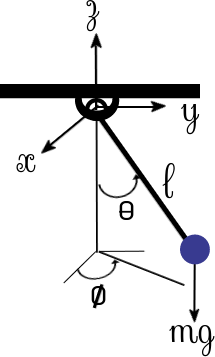
\includegraphics[scale=0.6]{problema5fig1}
 \caption{Péndulo esférico.}
 \label{fig:problema5fig1}
\end{figure}

recordamos que para el péndulo esférico la lagrangiana se escribe como 

\begin{equation}
 L = T - V = \frac{1}{2}ml^2(\dot{\theta}^2 + \dot{\phi}^2\sen^2{\theta} 
 - mgl\cos{\theta},
\end{equation}

podemos ahora escribir la hamiltoniana del sistema, primero obteniendo los momentos 
conjugados para las variables $\theta$ y $\phi$, 

\begin{equation}
 p_\theta = \frac{\partial L}{\partial \dot{\theta}} = ml^2\dot{\theta},
\end{equation}

\begin{equation}
 p_\phi = \frac{\partial L}{\partial \dot{\phi}} = ml^2\dot{\phi}\sen^2{\theta},
\end{equation}

de donde obtenemos 

\begin{equation}
 \dot{\theta} = \frac{p_\theta}{ml^2},
\end{equation}

y

\begin{equation}
 \dot{\phi} = \frac{p_\phi}{ml^2\sen^2{\theta}},
\end{equation}

y ahora utilizando 

\begin{equation}
 H = \sum_i p_i \dot{q}^2(q,p) - L, 
\end{equation}

la hamiltoniana del péndulo esférico resulta

\begin{equation}
 H = \frac{p_\theta^2}{2ml^2} + \frac{p_\phi^2}{2ml^2\sen^2{\theta}} 
 + mgl\cos{\theta}.
\end{equation}

Podemos notar ahora dos cosas. Primero, debido a que la coordenada $\phi$ es 
ignorable según la forma de la lagrangiana, entonces su momento conjugado se 
conservará, es decir que $p_\phi$ es constante, y además debido a que la energía 
cinética es una forma cuadrática de las velocidades y que la lagrangiana no depende 
explícitamente del tiempo, entonces la hamiltoniana es igual a la energía total 
del sistema, que también será una integral de movimiento. Usando la notación del
método de Liouville, podemos escribir esto de la siguiente forma 

\begin{equation}
  \frac{p_\theta^2}{2ml^2} + \frac{p_\phi^2}{2ml^2\sen^2{\theta}} 
 + mgl\cos{\theta} = I_1 = E,
 \label{eq:energiaPendEsf}
\end{equation}

\begin{equation}
 p_\phi = I_2.
 \label{eq:pphiPendEsf}
\end{equation}

Ahora hemos encontrado entonces dos integrales de movimiento, nos preguntamos ahora 
si están en involución, es decir si 

\begin{equation}
 \{I_1, I_2\} = 0,
\end{equation}

para ver esto recordamos la expresión para los paréntesis de Poisson, 

\begin{equation}
 \frac{\partial I_1}{\partial \theta}\cancelto{0}{\frac{I_2}{\partial p_\theta}} 
 - \frac{\partial I_1}{\partial p_\theta}\cancelto{0}{\frac{I_2}{\partial \theta}} + 
 \cancelto{0}{\frac{\partial I_1}{\partial \phi}}\frac{I_2}{\partial p_\phi} 
 - \frac{\partial I_1}{\partial p_\phi}\cancelto{0}{\frac{I_2}{\partial \phi}} = 
 0.
\end{equation}

Por lo tanto hemos demostrado que las dos integrales de movimiento que hemos encontrado 
están en involución, y debido a que hay tantas integrales de movimiento en involución como grados 
de libertad el sistema es integrable. Esto quiere decir que la uno forma $\omega = 
\sum_i p_idq^i$, que en términos de nuestras coordenadas y definiciones tiene la 
forma (despejando $p_\theta$ de \eqref{eq:energiaPendEsf}),

\begin{equation}
 \omega = \sqrt{2ml^2\left(I_1 - mgl\cos{\theta} - \frac{1}{2}\frac{I_2}{ml^2\sen^2{\theta}}
 \right)}d\theta + I_2d\phi,
\end{equation}

utilizando el teorema de Liouville es integrable, y al integrarla obtenemos 

\begin{equation}
 F = \int \sqrt{2ml^2\left(I_1 - mgl\cos{\theta} - \frac{1}{2}\frac{I_2}{ml^2\sen^2{\theta}}
 \right)}d\theta + I_2\phi.
\end{equation}

Y en vistas del mismo teorema podemos ver entonces a $F(q,I)$ como una función 
generadora de tipo dos, que al complementarla con 

\begin{equation}
 Q^i = \frac{\partial F(q,I)}{\partial I_i},
 \label{eq:QiPendEsf1}
\end{equation}

obtenemos una transformación canónica de coordenadas 

\begin{equation}
 (q,p) \leftrightarrow (Q,I),
\end{equation}

que nos lleva a un sistema canónico de coordenadas donde los impulsos son las 
integrales de movimiento. Ahora calculando las $Q^i$ utilizando \eqref{eq:QiPendEsf1}, 
obtenemos 

\begin{equation}
 Q^1 = \frac{\partial F}{\partial I_1} = \int \frac{ml^2}{\sqrt{2ml^2\left(I_1 -
 mgl\cos{\theta} - \frac{1}{2}\frac{I_2}{ml^2\sen^2{\theta}} \right)}}d\theta,
 \label{eq:Q1PendEsf1}
\end{equation}

\begin{equation}
 Q^2 = \phi - \int \frac{I_2}{\sen^2{\theta}\sqrt{2ml^2\left(I_1 - mgl\cos{\theta} - 
 \frac{1}{2}\frac{I_2}{ml^2\sen^2{\theta}} \right)}}d\theta.
 \label{eq:Q2PendEsf2}
\end{equation}

Y en nuestro nuevo sistema canónico $(Q^1,Q^2,I_1,I_2)$ tenemos 

\begin{equation}
 H = I_1 = E,
\end{equation}

por lo que 

\begin{equation}
 \dot{Q}^1 = \frac{\partial H}{\partial I_1} = 1,
\end{equation}

y 

\begin{equation}
 \dot{Q}^2 = \frac{\partial H}{\partial I_2} = 0.
\end{equation}

Y de estas ecuaciones podemos escribir, llamando a las constantes de integración 
$\beta^1$ y $\beta^2$ respectivamente, 

\begin{equation}
 Q^1 = t + \beta^1,
\end{equation}

\begin{equation}
 Q^2 = \beta^2,
\end{equation}

y utilizando estos resultados las ecuaciones \eqref{eq:Q1PendEsf1} y \eqref{eq:Q2PendEsf2}, 
quedan como 

\begin{equation}
 \boxed{t = -\beta^1 + \frac{\partial F}{\partial I_1} = \int \frac{ml^2}{\sqrt{2ml^2\left(I_1 -
 mgl\cos{\theta} - \frac{1}{2}\frac{I_2}{ml^2\sen^2{\theta}} \right)}}d\theta.}
\end{equation}

\begin{equation}
 \boxed{\phi = \beta^2 + \int \frac{I_2}{\sen^2{\theta}\sqrt{2ml^2\left(I_1 - mgl\cos{\theta} - 
 \frac{1}{2}\frac{I_2}{ml^2\sen^2{\theta}} \right)}}d\theta.}
\end{equation}

Con lo cual hemos reducido el péndulo esférico a cuadraturas utilizando el método 
de Liouville.

\begin{thebibliography}{10}
\bibitem{rashed}
R. Rashed, \emph{“Géométrie et dioptrique au Xe siècle: Ibn Sahl, 
Al-Quhi et Ibn Al-Haytham}, Las Belles Lettres, 1993.
\bibitem{holm}
D. Holm, \emph{Geometric Mechanics, Part I: Dynamics and Symmetry}, World Scientific, 
Imperial College Press, 2008.
\bibitem{romer}
H. Römer, \emph{Theoretical Optics: An introduction}, Wiley-VCH, 2005.
\bibitem{abraham}
 R. Abraham y J. Marsden, \emph{Foundations of Mechanics}, 2da edición, Addison-Wesley,
 1978.
\end{thebibliography}

\end{document}